\section{Analysis of the results}
In this section we are going to discuss the results of the top-k algorithm applied to the IMDb graphs. We are particularly interested in two factors:
\begin{itemize}
    \item The time needed to for the execution in function of different filtering values.
    \item The discrepancy on the results while varying the filtering values
\end{itemize}
The first one will tell us how much more efficient the algorithm is in terms of time, independently from the results. The second one is the metric to understand how accurate the filtered algorithm is. It's clear that even if we can compute the algorithm 100 times faster, it's of no use if the results are completely different from the real ones.\s

\nd The platform for the tests is \emph{a laptop}, so can not be considered precise due factors as thermal throttling. The CPU is an Intel(R) Core™ i7-8750H (6 cores, 12 threads), equipped with 16GB of DDR4 @2666 MHz RAM.

\subsection{Actors graph} \label{actors-graph}
Let's take into analysis the graph were each actors is a node and two nodes are linked the if they played in a movie together. In this case, during the filtering, we created the variable \texttt{MIN\textunderscore ACTORS}. This variable is the minimun number of movies that an actor/actress has to have done to be considered in the computation. \s

\nd Varying this variable obviously affects the algorithm, in different ways. The higher this variable is, the less actors we are taking into consideration. So, with a smaller graph, we are expecting better results in terms of time execution. On the other hand, we also can expect to have less accurate results. What we are going to discuss is how much changing \texttt{MIN\textunderscore ACTORS} affects this two factors.

\subsubsection{Time of execution} \label{time-actors}

In this section we are going to analyze the performance of the algorithm in function of different values of \texttt{MIN\textunderscore ACTORS}. Low values of this variable will lead to and exponential growth of the cardinality of the nodes and edges set cardinality.
\newpage

\begin{figure}[h!]
    \centering
    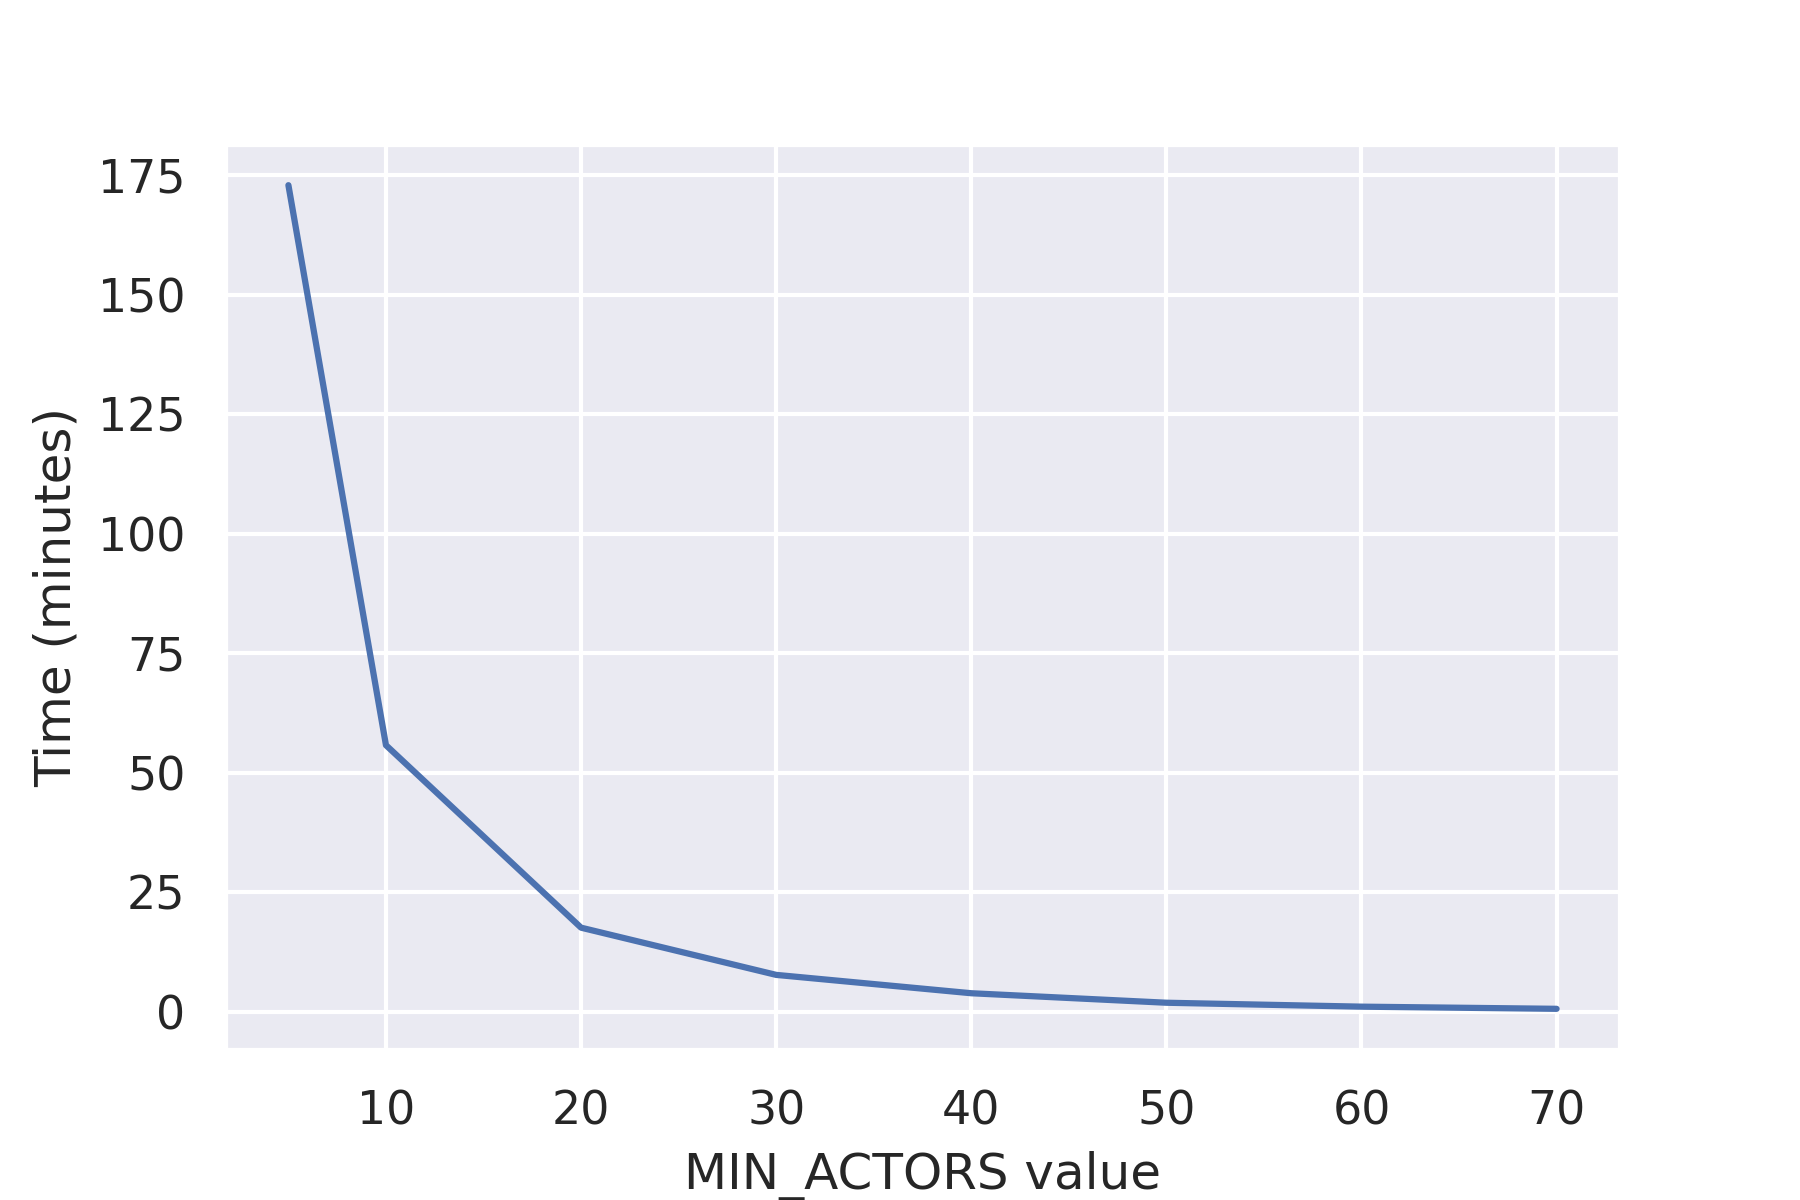
\includegraphics[width=12cm]{actors_time.png}
    \caption{\emph{CPU time} in relation to the \texttt{MIN\textunderscore ACTORS} variable}
    \label{fig:actors_time}
\end{figure}

\nd In figure \ref{fig:actors_time} it's only taken into consideration the \emph{CPU time} (divided by the number of threads). However, \emph{system time} is in the order of a few minutes in the worst case.

\subsubsection{Variation of the nodes and edges cardinality}

Let's analyze how much this filtering effects our data. While varying the variable for the filtering, we are changing the condition for a node to be considered or not.

\begin{table}[h!]
    \centering
     \begin{tabular}{||c c c||}
     \hline
     \texttt{MIN\textunderscore ACTORS} & Number of nodes & Number of Edges \\ [0.5ex]
     \hline\hline
     1 & 923109 & 3202679 \\
     5 & 126771 & 1949325 \\
     15 & 37955 & 1251717 \\
     20 & 26337 & 1056544 \\
     31 & 13632 & 748580 \\
     42 & 7921 & 545848 \\ [1ex]
     \hline
     \end{tabular}
    \label{table:actors}
\end{table}

\nd In \ref{table:actors} we can the exponential growth of both nodes and edges cardinality with lower values of \texttt{MIN\textunderscore ACTORS}. This explains clearly the results obtain in \ref{time-actors}

\subsubsection{Discrepancy of the results}
We want to analyze how truthful our results are while varying \texttt{MIN\textunderscore ACTORS}. The methodology is simple: for each results (lists) we take the intersection of the two. This will return the number of elements in common. Knowing the length of the lists, we can find the number of elements not in common. \s

\nd A way to see this results is with a square matrix $n \times n, ~ A = (a_{ij})$, where $n$ is the number of different values that we gave to \texttt{MIN\textunderscore ACTORS} during the testing. In this way the $(i,j)$ position is the percentage of discrepancy between the results with \texttt{MIN\textunderscore ACTORS} set as $i$ and $j$ \s

\nd This analysis is implemented in python using the \texttt{pandas} and \texttt{numpy} libraries.

\lstinputlisting[language=c++]{code/closeness_analysis.py}

\nd Visualizing it we obtain the matrix in figure \ref{fig:matrix-a}. As expected, it is symmetrical and the elements on the diagonal are all equal to zero. We can see clearly that with a lower value of \texttt{MIN\textunderscore ACTORS} the results are more precise. The discrepancy with \texttt{MIN\textunderscore ACTORS=10} is 14\% while being 39\% when \texttt{MIN\textunderscore ACTORS=70}.

\begin{figure}[h!]
    \centering
    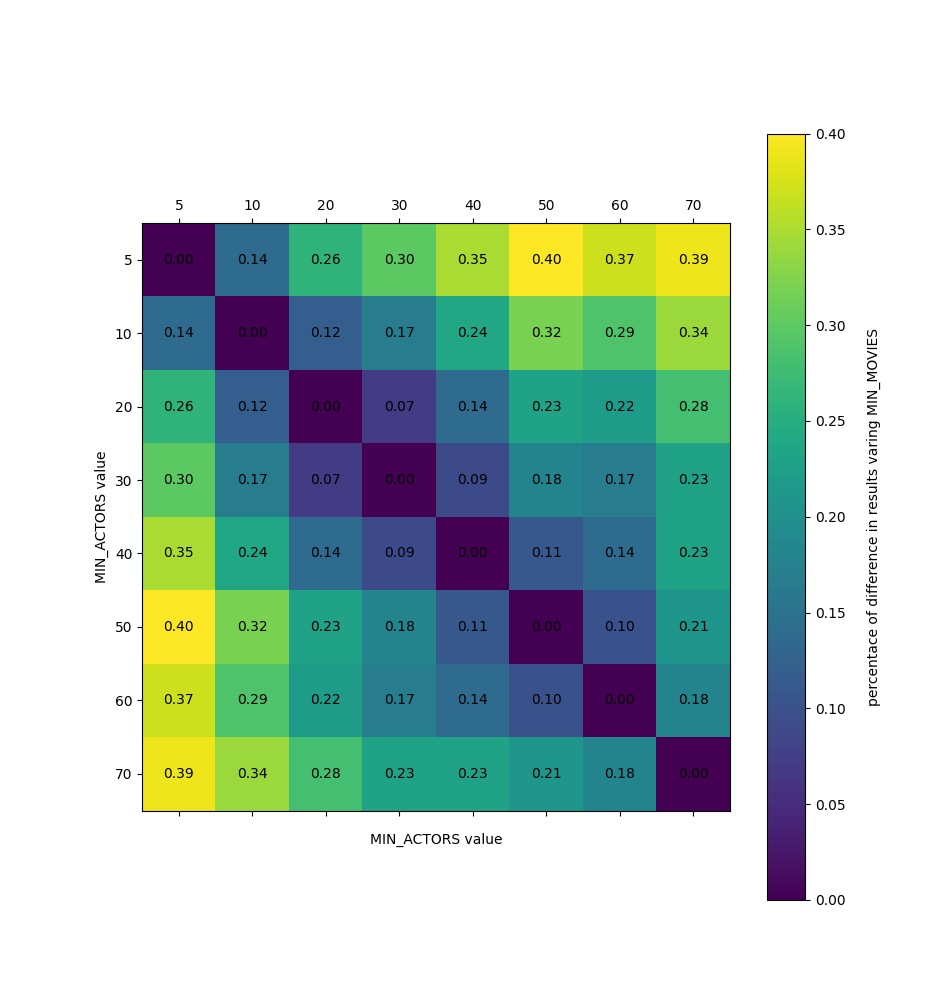
\includegraphics[width=11.5cm]{Figure_1.png}
    \caption{Discrepancy of the results on the actors graph in function of the minimum number of movies required to be considered as a node}
    \label{fig:matrix-a}
\end{figure}
\s
\nd This is what we obtain confronting the top-k results when $k=100$. It cloud be interesting to see how much the discrepancy changes with different values of $k$. However, choosing a lower value for $k$ would not be useful for this type of analysis. Since we are looking at the not common elements of two lists, with a small length, we would get results biased by statistical straggling. \s

\s
\newpage
\subsection{Movies Graphs}
In this section we are taking into consideration the graph build over the movies and their common actors/actresses. Due to an elevated number of nodes, to optimize the performance, in section \ref{filtering} we introduced the variable \texttt{VOTES}. It represents the minimum number of votes (indifferently if positive or negative) that a movie needs to have on the IMDb database to be considered as a node in our graph.

As seen during the analysis of the actors graph in \ref{actors-graph}, varying this kind of variables affects the results in many ways.

\subsubsection{Time of execution}

As seen in \ref{time-actors} we are going to analyze the performance of the algorithm in function of different values of \texttt{VOTES}. Low values of this variable will lead to and exponential growth of the cardinality of the nodes and edges set cardinality. And as we know, with a bigger graph there are more operations to do. The results are shown in figure \ref{fig:moves_time}

\begin{figure}[h!]
    \centering
    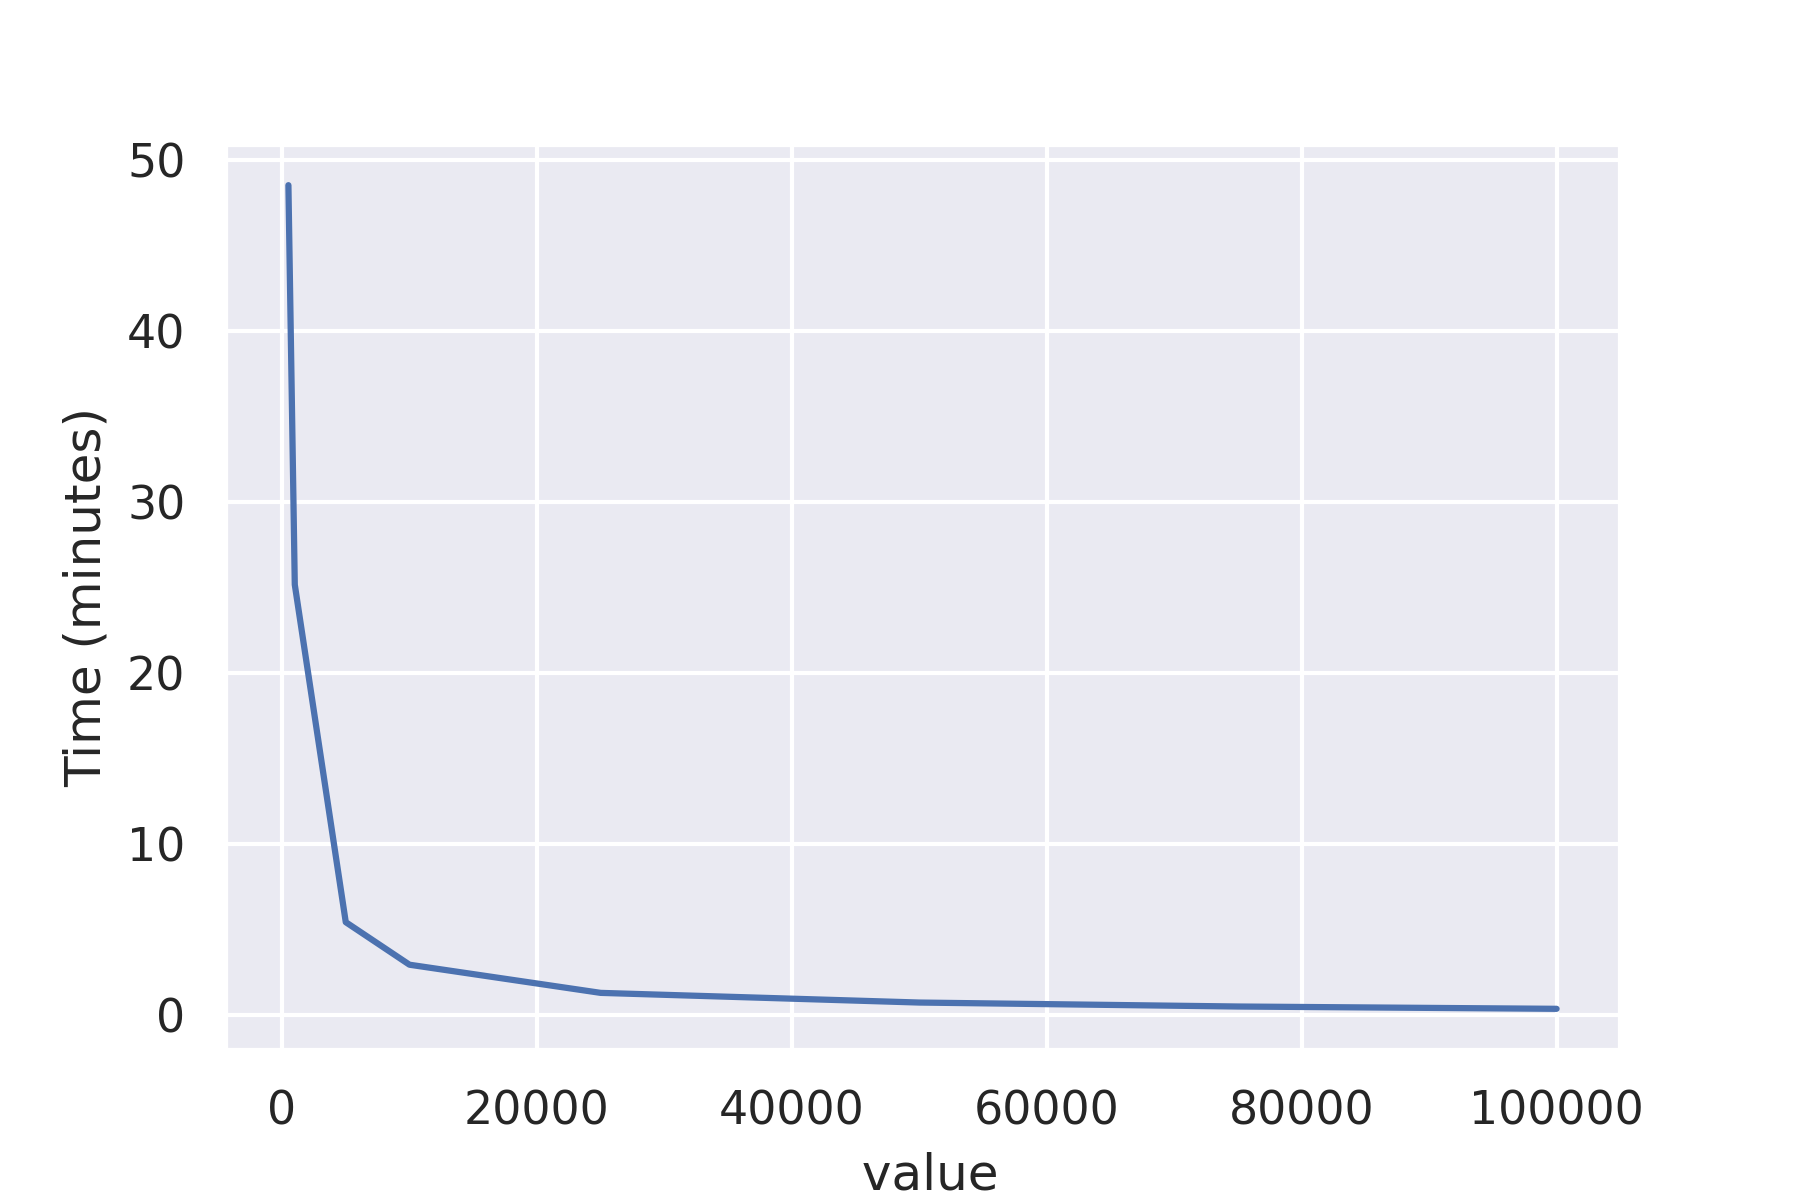
\includegraphics[width=12cm]{movies_time.png}
    \caption{\emph{CPU time} in relation to the \texttt{VOTES} variable}
    \label{fig:moves_time}
\end{figure}

\newpage


\subsubsection{Discrepancy of the results}

All the observations made before are still valid for this case, I won't repeat them for shortness. As done before (\ref{fig:matrix-a}), we are going to use a matrix to visualize and analyze the results
\s

% \lstinputlisting[language=c++]{code/closeness_analysis_2.py}

\nd Giving us the matrix in figure \ref{fig:matrix-b}:
\begin{figure}[H]
    \centering
    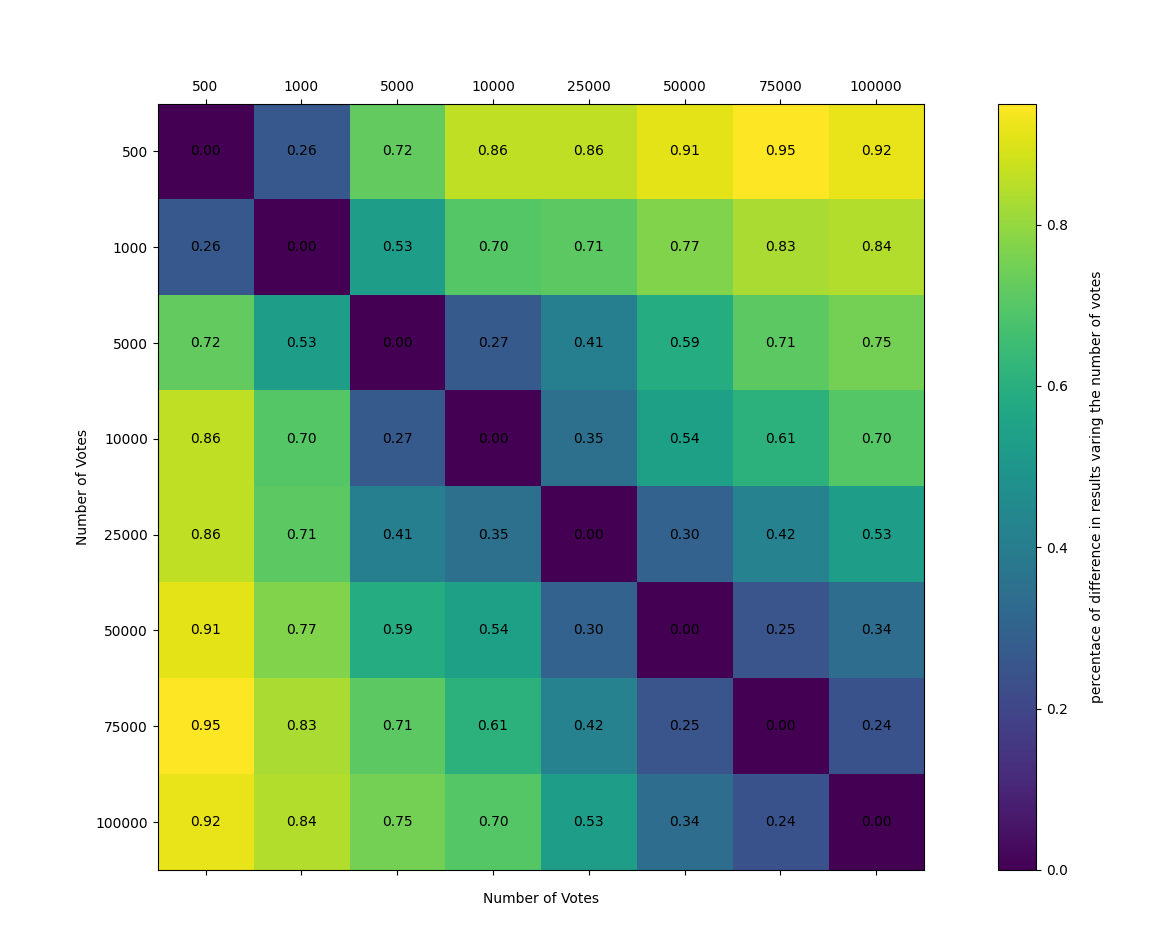
\includegraphics[width=13cm]{Figure_2.png}
    \caption{Discrepancy of the results on the movie graph in function of the minimum number of votes required to be considered as a node}
    \label{fig:matrix-b}
\end{figure}
\newpage
\lstinputlisting[language=c++]{code/closeness_analysis_2.py}

\s \nd In this graph there is much more discrepancy in the results with a lower cardinality of the node's set. Even if the lowest and biggest value of \texttt{VOTES} give us a graph with the same order of nodes of the previous one, the percentage difference in accuracy is completely different. The reason to that is that those two graphs taken into example are very different. If we want an higher accuracy on the movies graph, we have to loose some performance and use lower values of \texttt{VOTES}.
